\section{Schéma zapojení LNA}
	LNA Low Noise Amplifer, neboli nízkošumový zesilovač, je zesilovač určený k zesílení signálu z antény. tento zesilovač je selektivní, díky vstupnímu filtru pásmové propusti. Tento elektronický obvod tedy do značné míry určuje možnosti zařízení.
	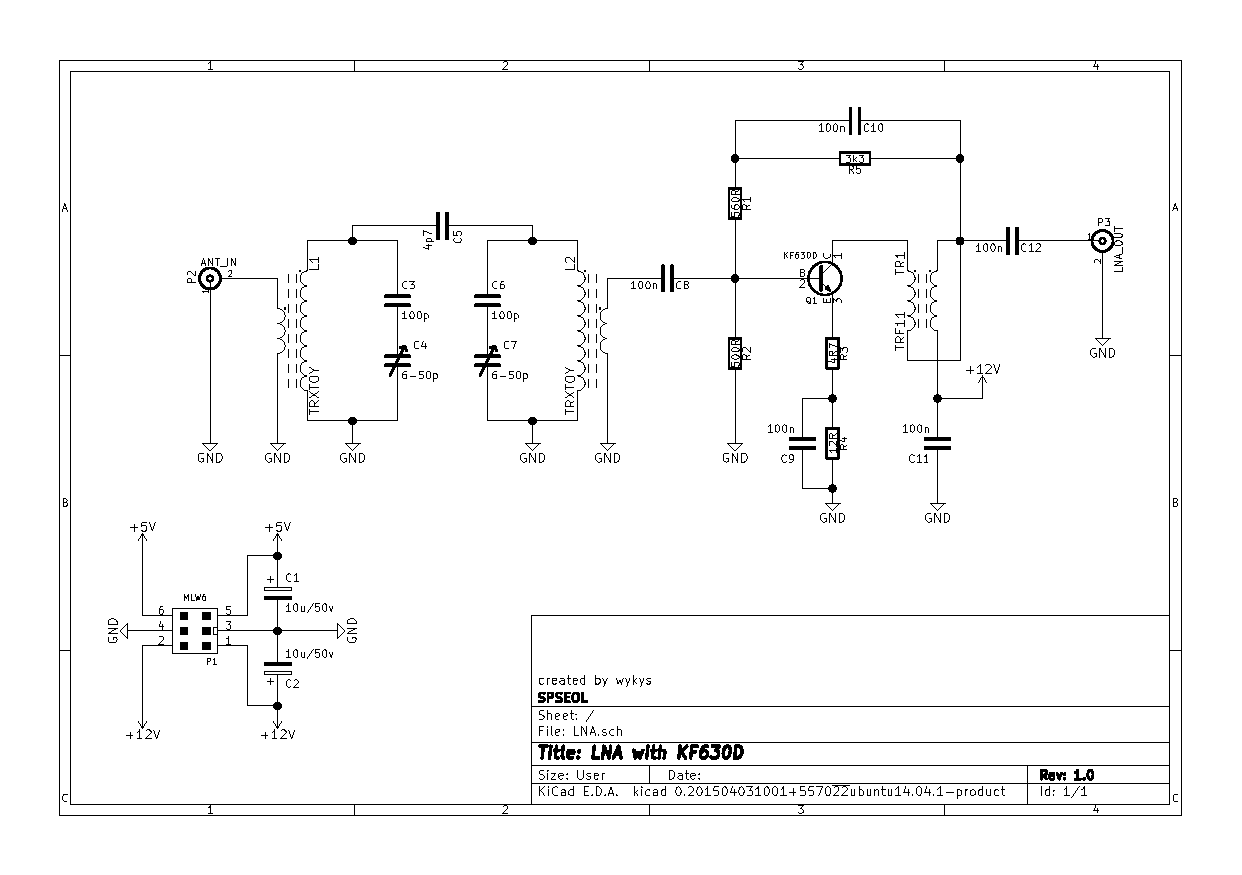
\includepdf[landscape=true]{img/LNA.pdf}
	
\section{Schéma zapojení DDS}
	Schéma je rozděleno do tří bloků v levé horní části se nachází stabilizátor 3V3 pro křemíkový oscilátor a Kondenzátory pro vyrovnání nárazových odběrů. V levé dolní části je digitální část DDS, popisováno z leva do prava: konektor pro konfigurování DDSky, oddělovací buffer 74F245, jehož výstupy jdou do DDSky. Nahoře je již zmíněný křemíkový oscilátor a tvarovač impulsů. V pravé horní části se nachází VF část tvořená dolní propustí určené k potlačení vyšších harmonických z DAC. a Výkonový zesilovač tvořený tranzistorem KF630D s I$_c$ nastaveným na $20~mA$. Ke kolektoru tranzistoru je připojeno trafo, které je vinuto bifilárně a slouží k transformaci impedance na cca $50~\Omega$.
	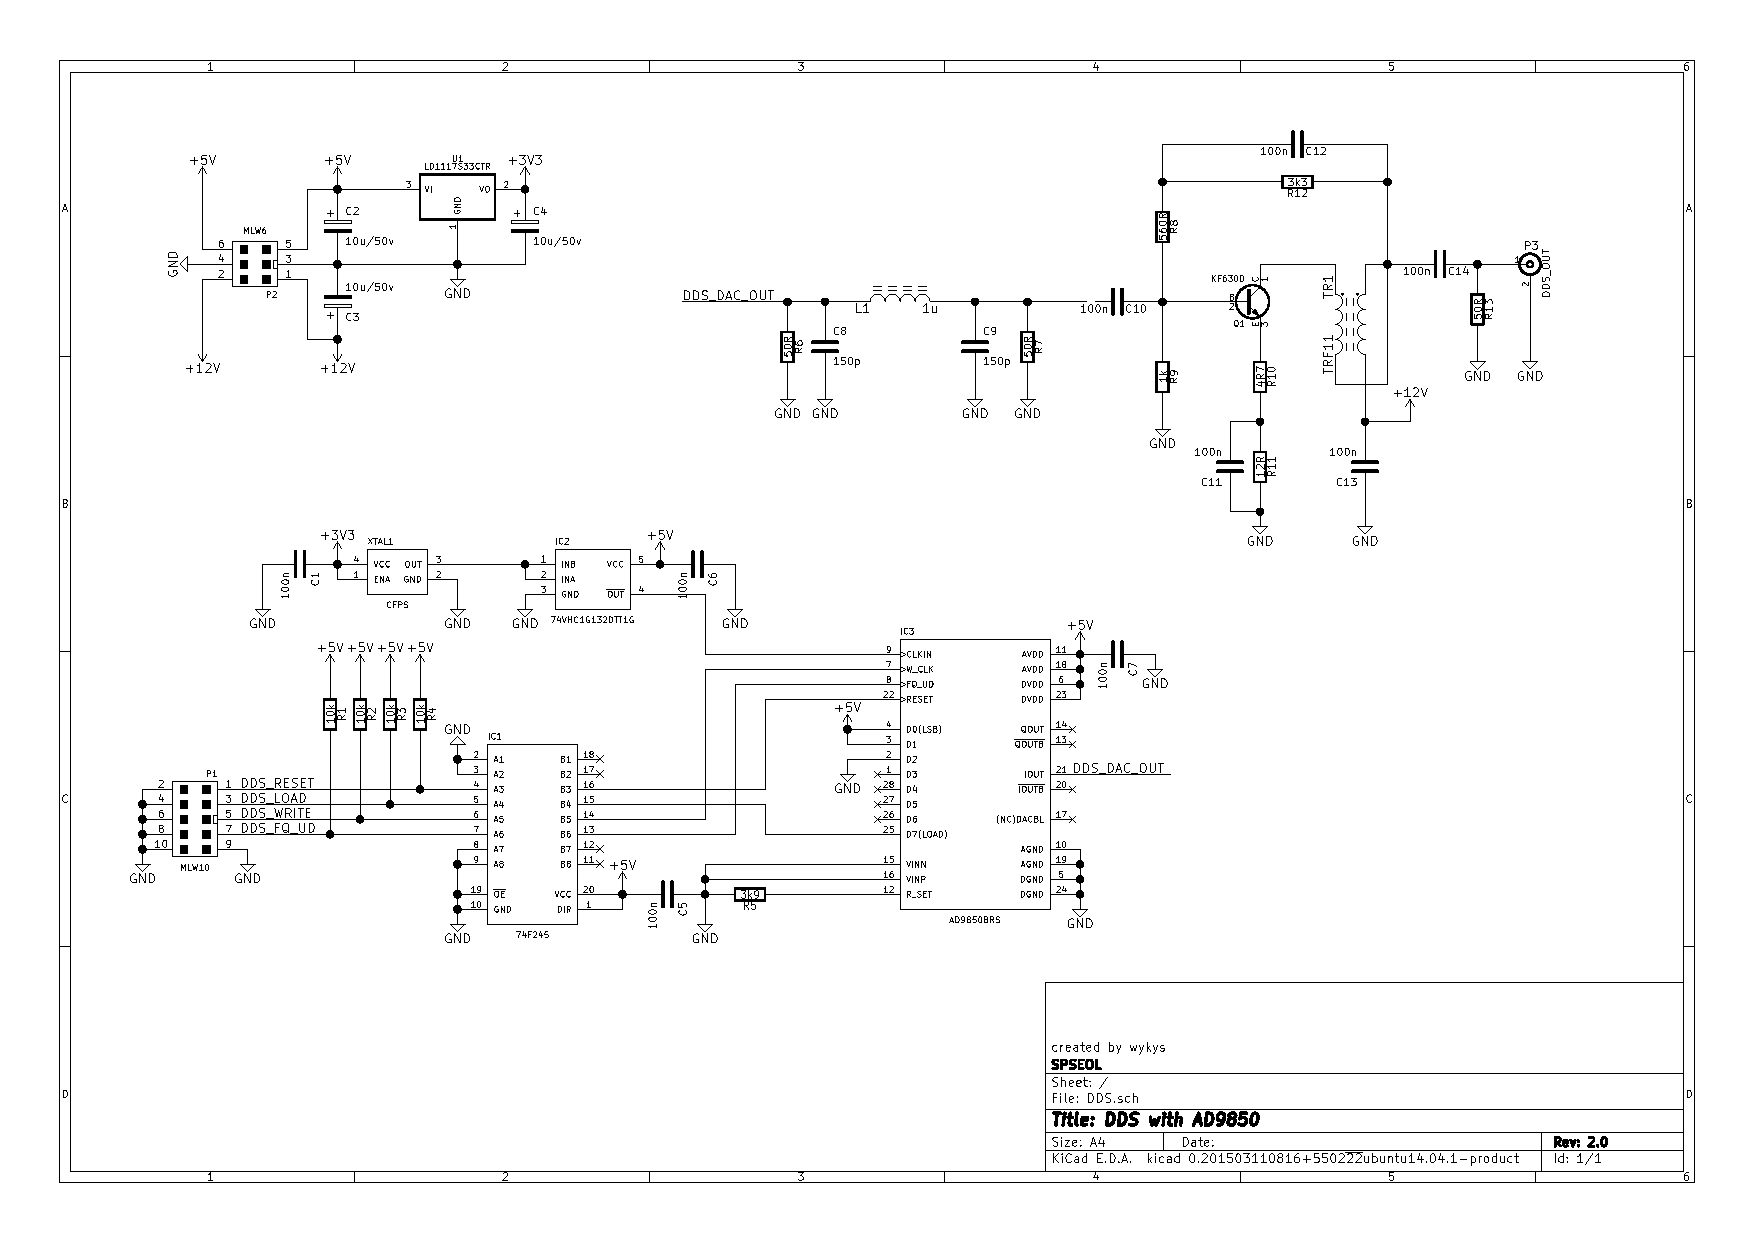
\includepdf[landscape=true]{img/DDS.pdf}
	
\section{Schéma zapojení řídící deska}
	Řídící deska slouží k řízení výstupní frekvence lokálního oscilátoru založeného na DDS. A nastavování pořadované výstuúní frekvence slouží enkoder. Dále je na desce připraven konektor pro USART, aby bylo možné řídit i řídíví desku s nadřazeného počítače. Dále desky zobraduje příjmanou stanici na znakový LCD disply. Zobrazovaná frekvence je absolutní hodnota zordílu frekvence lokálního oscilátoru a mezifrekvence.
	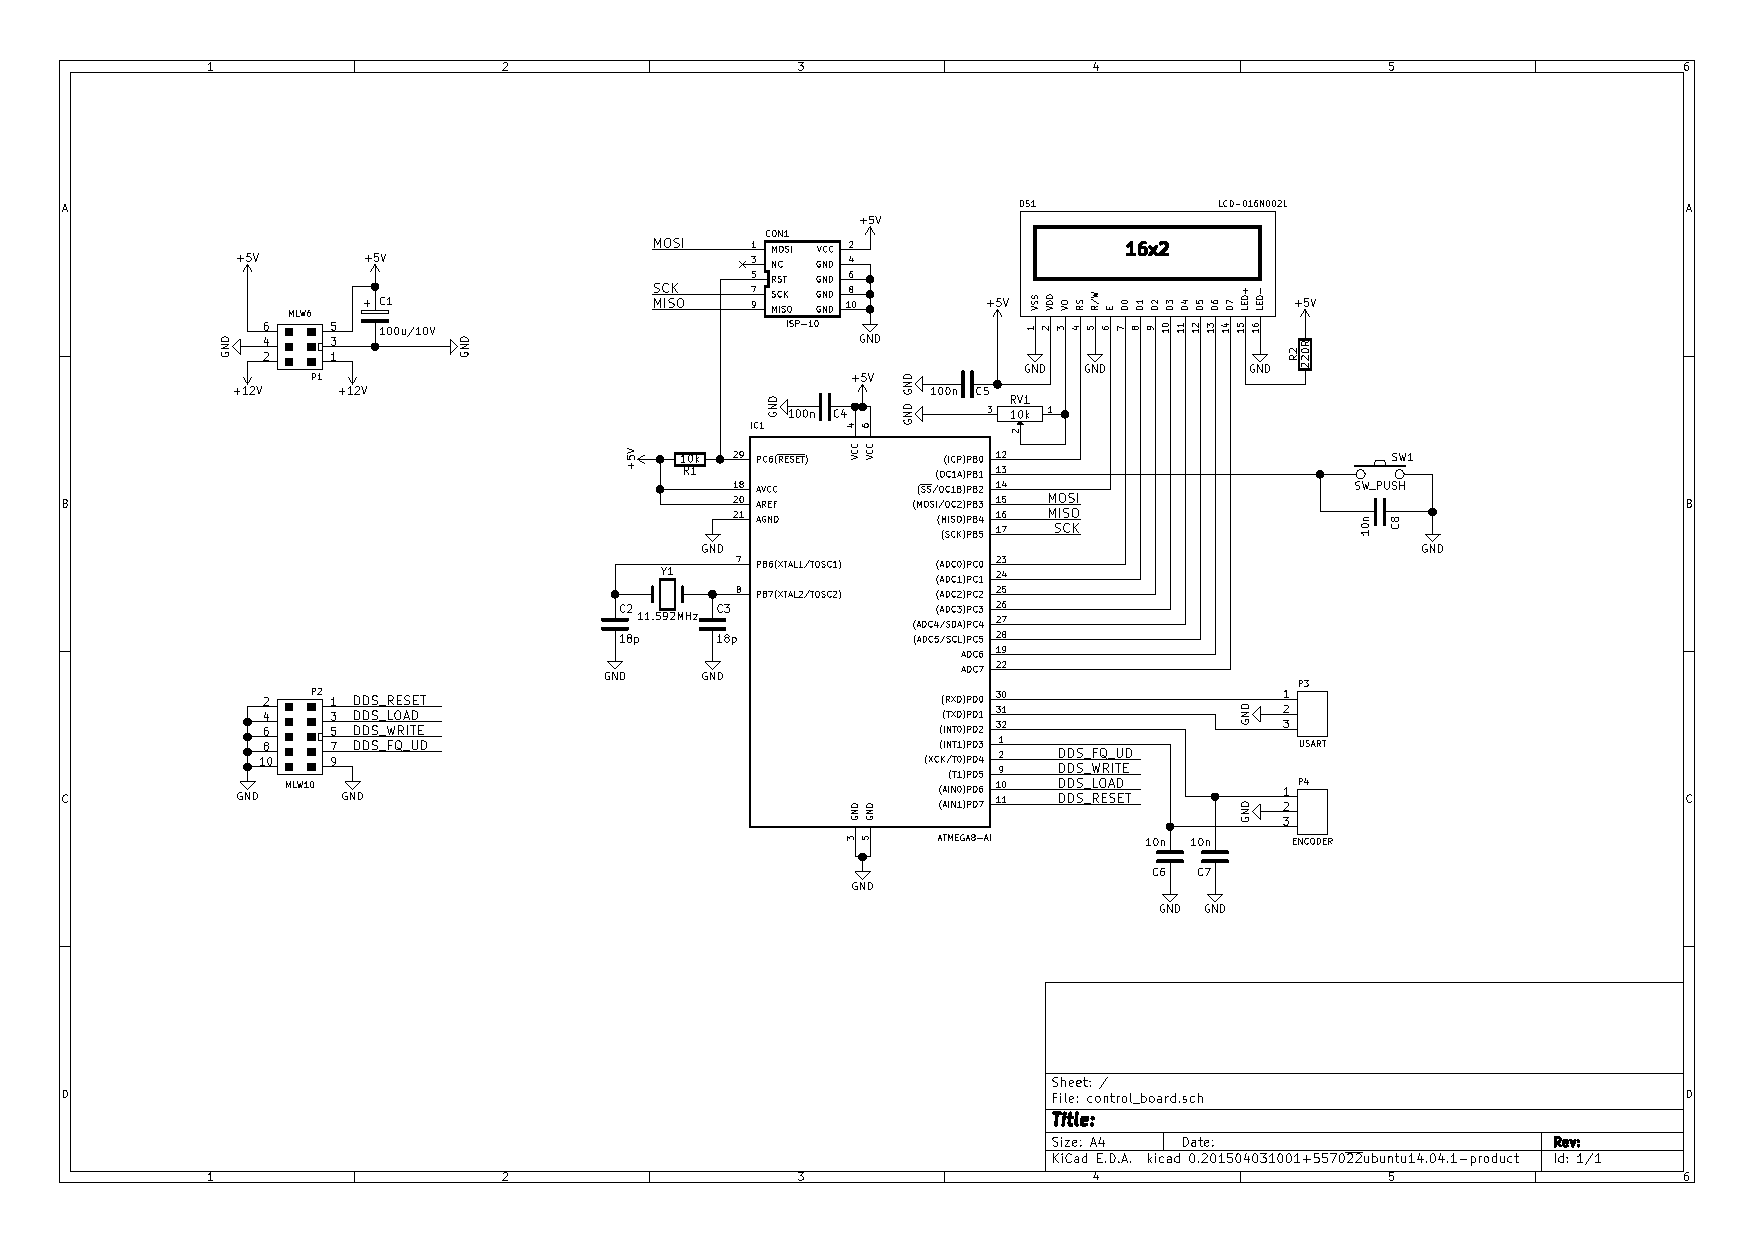
\includepdf[landscape=true]{img/control_board.pdf}
	
\section{Schéma zapojení mixer}
	Tento obvod slouží k převedení signálu do základního pásma. K tomu používá dvou směšovaců. Klasického kruhového diodového směčovaře pro převod na mezifrekvenci $6~MHz$ a tzv. Tayloe kvadraturní detektor, který generuje signály I a Q navzájem posunuté o $\frac{\pi}{2}$.
	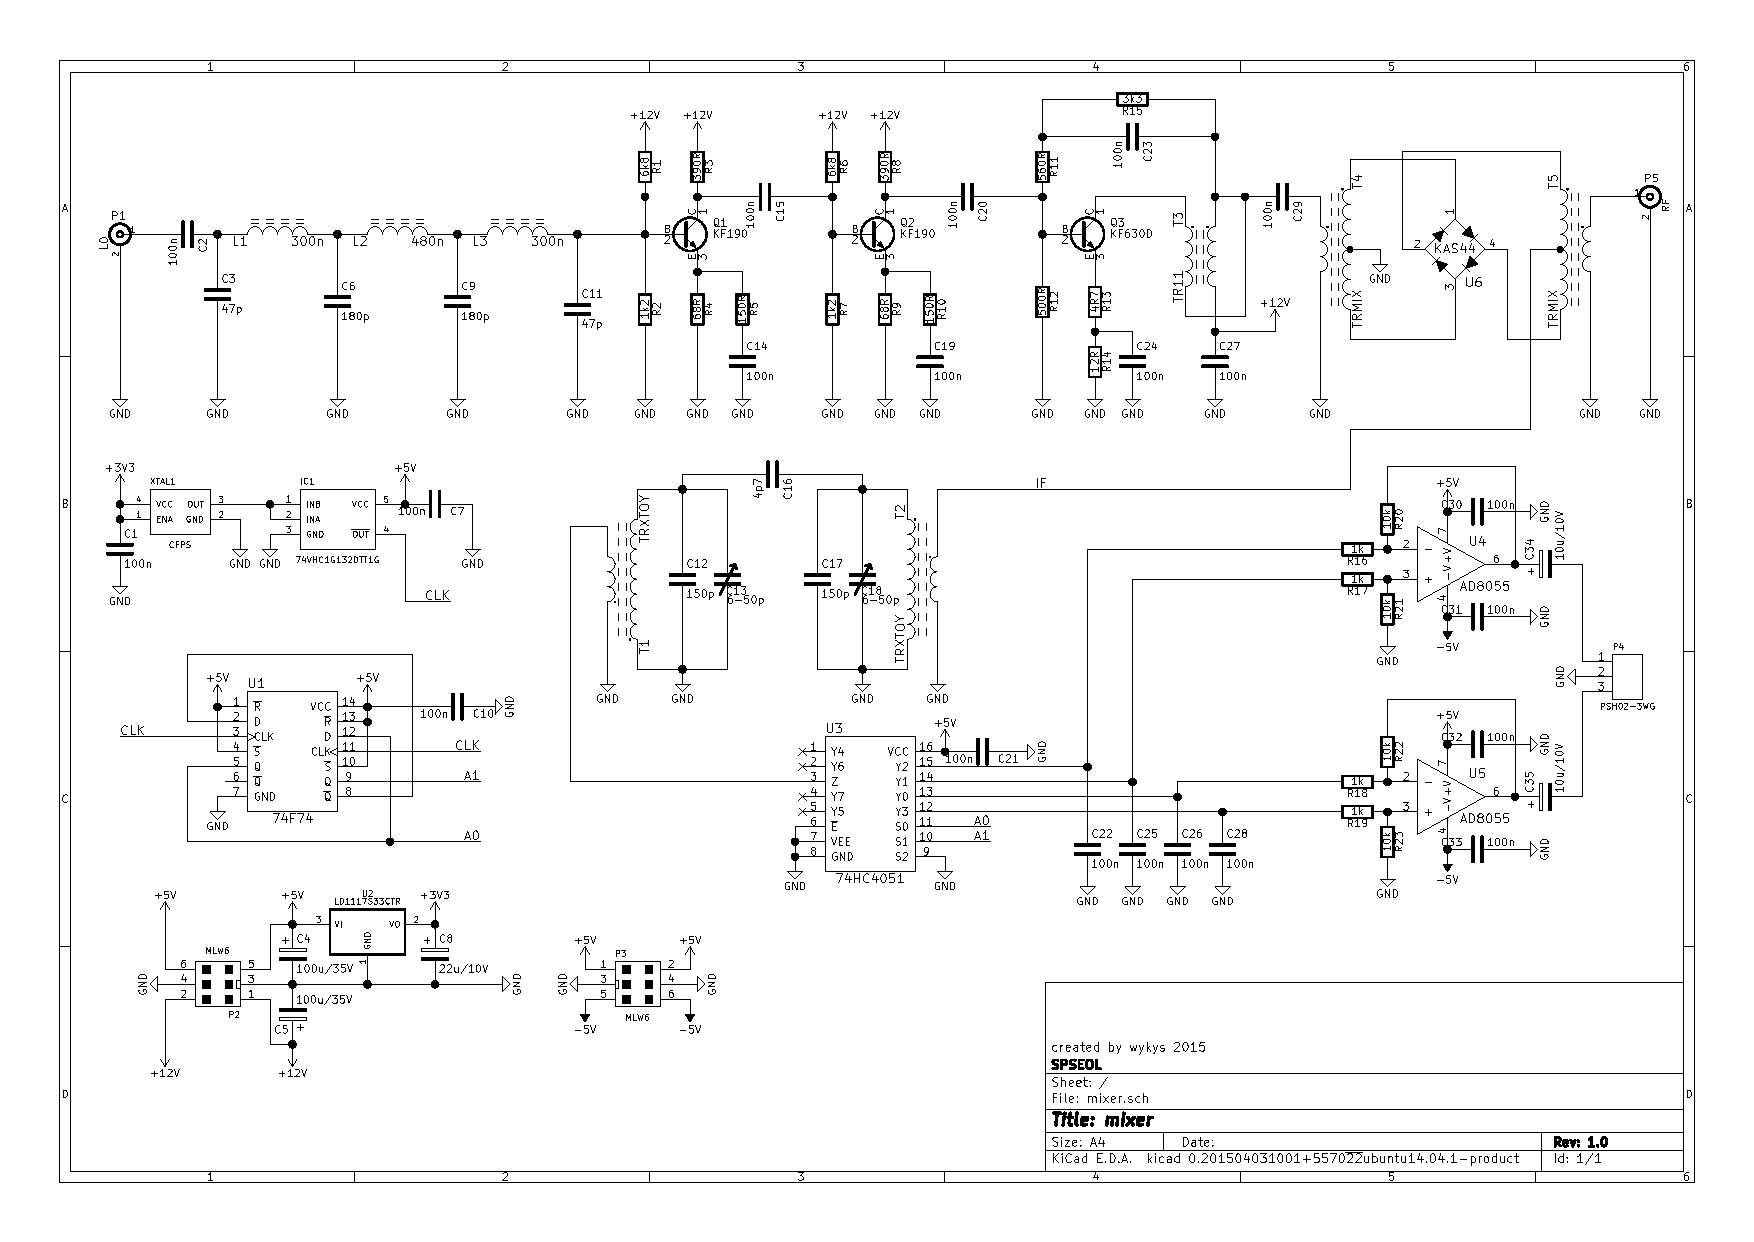
\includepdf[landscape=true]{img/mixer.pdf}
	
\section{Schéma zapojení zdroj}
	Zdroj slouží k napájení celého zařízení poskytuje symetrické napětí $5~V$ a napěří $12~V$.
	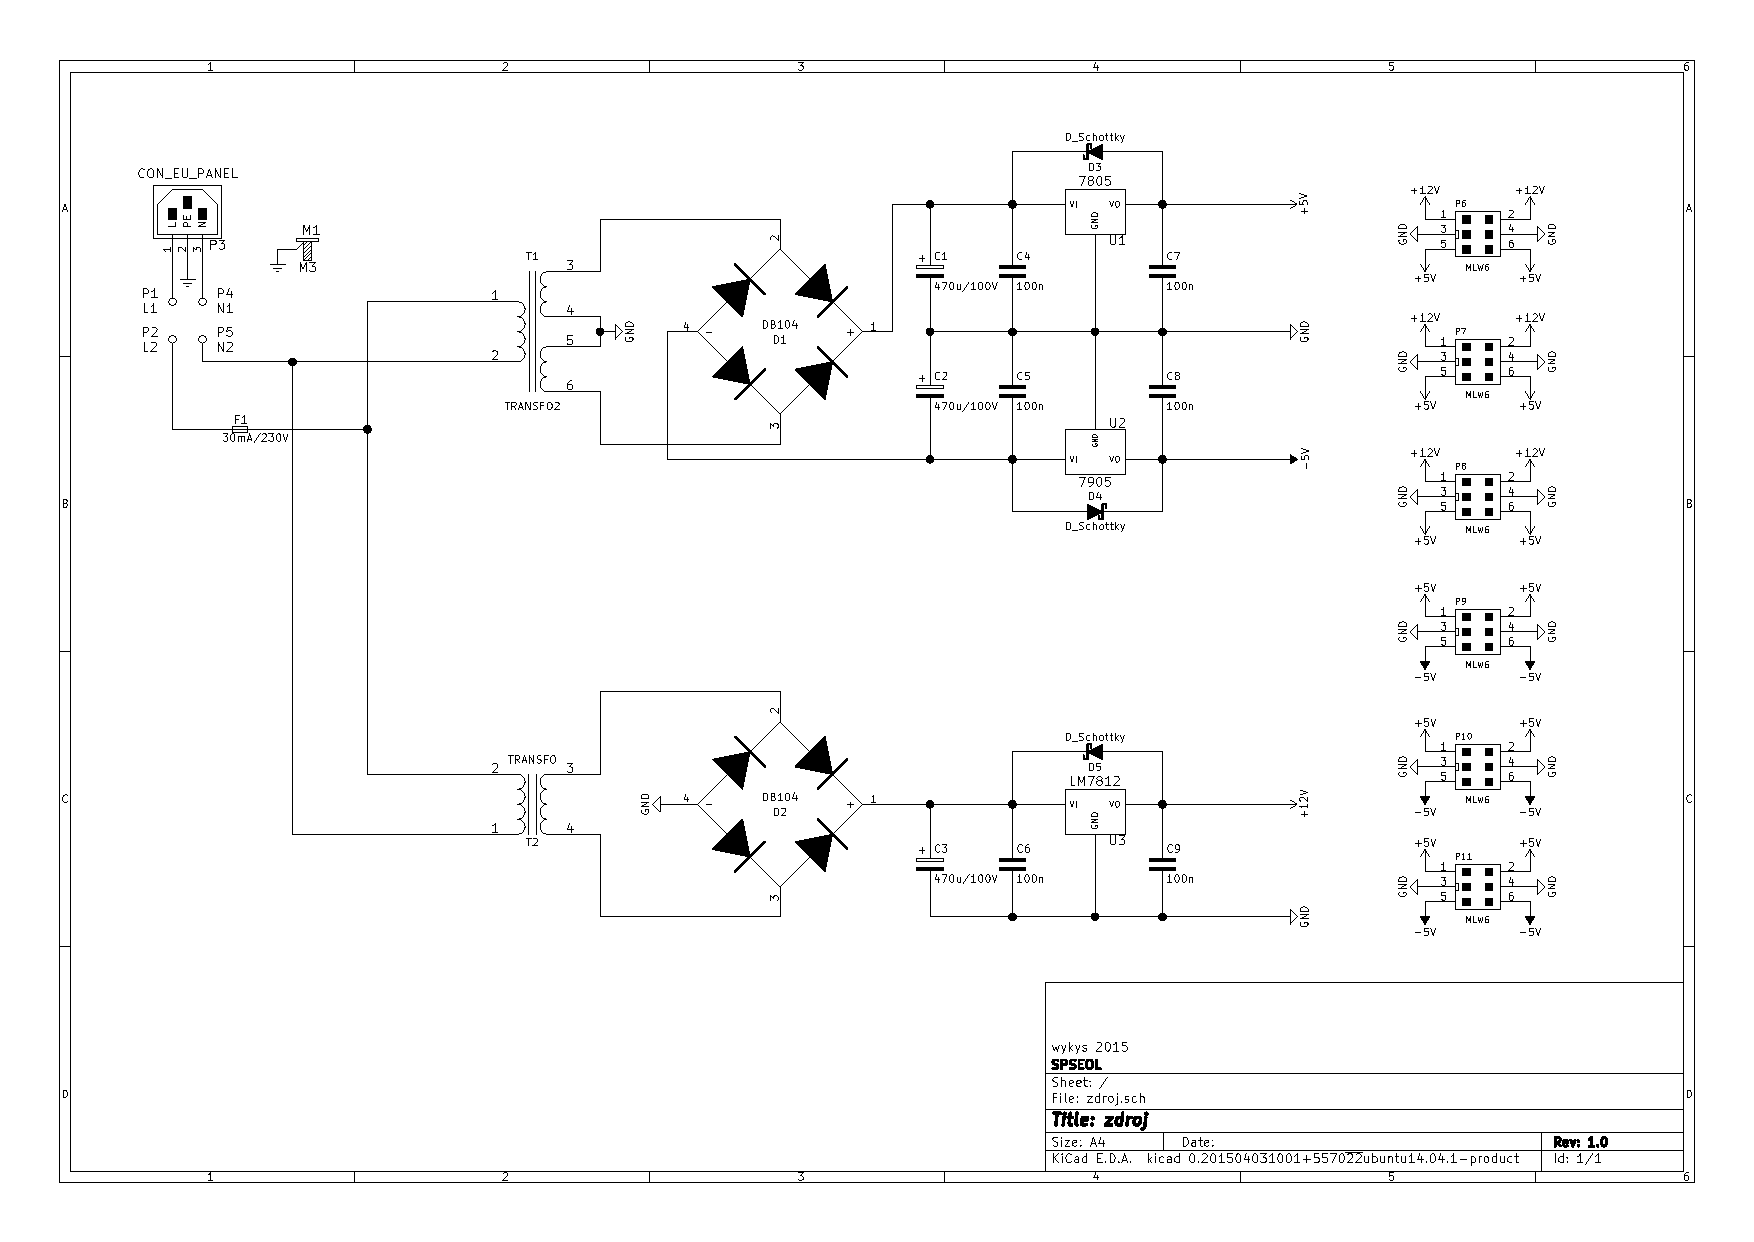
\includepdf[landscape=true]{img/zdroj.pdf}